%!TEX root = ../diploma.tex

\section{Обзор литературы}\label{sec:literature}
\subsection{Задача оптимизации памяти}

На Рис.~\ref{fig:cfg} приведен пример АГВ: можно заметить, что, например,
выделенные блоки памяти для следующих пар тензоров:
\begin{itemize}[nosep]
    \item $(t_2,t_3),(t_5,t_6)$ — не могут пересекаться независимо от выбора ТС
    \item $(t_1,t_4),(t_1,t_5),(t_3,t_6)$ — могут пересекаться независимо от
    выбора ТС
    \item $(t_2,t_4),(t_4,t_6)$ — могут пересекаться, если размерности
    соответствующих входов и выходов совпадают для операций \textbf{add} и
    \textbf{tanh}, поскольку они являются поэлементными операциями
    \item $(t_3,t_4)$ — могут или не могут пересекаться в зависимости от ТС
    (необходимо ли хранить значение $t_3$ после вычисления операции
    \textbf{add}) и совпадения размерностей $t_3$ и $t_4$
\end{itemize}
На Рис.~\ref{fig:ints} для этого примера приведена одна из возможных
топологических сортировок и помечены времена жизни для тензоров.

\begin{figure}[ht]
\centering
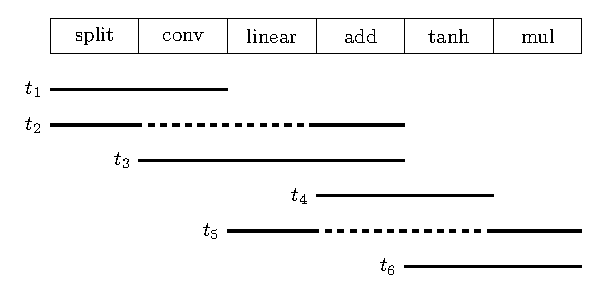
\includegraphics[scale=1.1]{ints}
\caption{Время жизни тензоров}
\label{fig:ints}
\end{figure}


Задача~\ref{eqn:opt} является NP-полной в случае различных размеров тензоров и
сводится, например, к задаче 3-разбиений~\cite{np_complete}. Тем не менее
возможен поиск приближенного решения эвристическими
алгоритмами~\cite{sekiyama2018profile},~\cite{pisarchyk2020efficient}.

В работе~\cite{sekiyama2018profile} задача~\ref{eqn:opt} выражается как частный
случай задачи упаковки прямоугольников (разместить прямоугольники в контейнер с
заданной шириной и наименьшей высотой), решаемый эвристическим алгоритмом. В
работе~\cite{pisarchyk2020efficient} для каждого тензора $t$ АГВ вычисляется
кратчайший отрезок вершин, включающий в себя все вершины, для которых $t$
является входящим или выходящим ребром (назовем его \textit{временем жизни}
$t$); тензорам $t_1$ и $t_2$ разрешено использовать общую память тогда и только
тогда, когда пересечение их времен жизни пусто. Далее описывается жадный
алгоритм, в котором перебираются тензоры по убыванию их размера, и для каждого
производится поиск наименьшего зазора в памяти, вмещающего его. Экспериментально
показывается, что описанная ими стратегия достигает результатов не хуже (иногда
лучше), чем эвристический метод из~\cite{sekiyama2018profile}, на примере
нескольких НС.

\subsection{Задача параллельных вычислений}
\label{subsec:literature:parallel}

Для разбиения множества вершин АГВ на непересекающиеся подмножества независимых
вершин можно использовать следующий подход, представляющий собой динамическое
программирование на ациклическом графе (предложен, например,
в~\cite{node_level_par}):
\begin{enumerate}
    \item Рассмотрим вершины графа в порядке топологической сортировки:
        \begin{itemize}
            \item если у очередной вершины $v$ нет входящих ребер,
            инициализируем $\variablename{maxdist}(v) = 0$;
            \item иначе, находим у вершины $v$ предка $w$ с наибольшим значением
            $\variablename{maxdist}(w)$, и затем инициализируем
            $\variablename{maxdist}(v) = \variablename{maxdist}(w)+1$.
        \end{itemize}
    \item Пусть $D=\max\limits_{v \in V}\variablename{maxdist}(v)$. Построим для
    вершин $V$ разбиение на подмножества: $\left\{L_0,\ldots,L_D\right\}$, где
    $L_i = \{v \mid \variablename{maxdist}(v) = i\}.$
\end{enumerate}
Будем называть $L_i, i\in\overline{0,D}$ слоями АГВ. Очевидно, $\forall
i,j\in\overline{0,D}\ i\not=j \rightarrow L_i \cap L_j = \emptyset$. Покажем,
что в каждом множестве находятся только попарно независимые вершины.

\newtheorem{statement}{Утверждение}
\numberwithin{statement}{section}
\begin{statement}
    \label{statement:maxdist}
    $\forall i\in\overline{0,D}\ \forall v,u \in L_i\ v$ и $u$ — независимы.
\end{statement}
\begin{proof}
    Допустим, что $v$ и $u$ не являются независимыми, то есть существует либо
    путь из $v$ в $u$, либо из $u$ в $v$. Но тогда длина наибольшего пути не
    может совпадать: в первом случае $\variablename{maxdist}(v) <
    \variablename{maxdist}(u)$, во втором $\variablename{maxdist}(u) <
    \variablename{maxdist}(v)$. Следовательно, если $v$ и $u$ принадлежат одному
    и тому же слою, то они независимы.
\end{proof}

Такой способ не гарантирует нахождения наибольших групп независимых вершин,
однако является вычислительно эффективным и для представлений НС в виде АГВ
находит приемлемое решение, что показано в разделе~\ref{sec:exp}.
